\documentclass{article}

\usepackage[
    backend=bibtex, 
    natbib=true,
    style=alphabetic,
    citestyle=alphabetic,
    maxcitenames=1,
    maxbibnames=99
]{biblatex}

\usepackage[utf8]{inputenc} 
\usepackage[T1]{fontenc}
\usepackage{lmodern}
\usepackage{graphicx}
\usepackage{tikz}
\usetikzlibrary{calc}
\usetikzlibrary{positioning}
\usepackage{url}
\usepackage{rotating}
\usepackage{graphicx}            % For pdf/bitmapped graphics files
\usepackage[margin=2cm]{geometry}
\graphicspath{{images/}}
\DeclareGraphicsExtensions{.pdf,.png,.jpg,.jpeg}

\addbibresource{roadmap.bib}
\usepackage{hyperref}

\begin{document}

\section{Introduction}

% Document: proposal to replace 2014 version: main issues identified
% - Difficult to plan long-term evolution in research -> guided by breakthrough
% - Example of kid-size
This document is a proposal to replace the roadmap proposed in 2014 for the
RoboCup humanoid
league~\footnote{\url{http://www.robocuphumanoid.org/wp-content/uploads/HumanoidLeagueProposedRoadmap.pdf}}. Criticism
have emerged with respect to establishing a long-term schedule for evolution of
the rules in a research context where evolution is mainly guided by breakthrough
rather than by linear development. Some of the changes planned revealed to be
difficult to implement: the removal of the KidSize initially planned for 2020
seems now unrealistic since this league still received more applications than
TeenSize and AdultSize together in 2019. Finally, the relationship between
missing skills and research topics was not explicited.

% Aim of this document
In order to avoid facing this issues, a different approach is used. Rather than
establishing a long-term schedule, the document describes the scientific challenges
for the league and the steps required to play against humans.
Upcoming changes in the next 5 years are described in more detail in order to allow
teams, local organizer and the RoboCup Federation to have a better insight on
evolution of the league.

% Gathering opinions
In order to produce a roadmap satisfying for both the trustees and the league,
a workshop was run at IROS2018 and polls have been proposed%
\footnote{Detailed results are available at~\url{http://www.labri.fr/perso/lhofer/content/robocup/roadmap_workshop_slides.pdf}}.
While a consensus was obtained on most of the questions,
this process has also shown that for some propositions it is difficult to reach an agreement.

% Document contains history and will be updated frequently
While the focus is on perspectives for the league,
the document also contains information on the history of the league,
thus allowing to improve understanding of the league evolution.
Updating this document regularly will allow to assess progress within the league
and ensure that modification to the rules are consistent with the level of the
teams.
An evolution of the rules consistent with the level of the teams and
scientific breakthrough is crucial to improve the attractivity of the league
for both researchers and public.

The structure of the documents is as
follows. Section~\ref{sec:ScientificChallenges} introduces the scientific
challenges related to the league and their importance in the games. The major
upcoming changes to the rules are presented in Section~\ref{sec:ShortTerm}. The
global evolution of the leagues is discussed in Section~\ref{sec:LongTerm}
through an event-triggered Roadmap and the history of changes which occured
since the creation of the league.

\section{\label{sec:ScientificChallenges}Scientific Challenges}

% TODO: introduction

\subsection{Issues in Motion Generation and Control of Humanoid Robots}

% Very brief history reminder
The first humanoid robot built was the WABOT-1 which was completed in 1972. 
While WABOT-1 was already able to walk, controlling the walking gait of a humanoid robot a challenging problem today. 
From designing dynamic walking gait to running and real-time adaptation of multi-objective motions, motion control of humanoid robots is an active research topic.

% Focus of RoboCup : introduction
While bipedal locomotion is still one of the main issues of the RoboCup humanoid
league in 2019, other motions are also important. 
At the moment these are mainly motions for standing up and kicking a ball on the ground.
In the future, this will also include jumps, headers, volleys, and other highly dynamic motions.
Given the adversarial nature of RoboCup, one of the key elements is also the transition between different motions in order to reduce the time required to achieve complex tasks. 
Finally, a major concern from a mechanical point of view are achieving satisfying performances while using low-cost hardware and ensuring the robustness of the hardware despite the fact that the robots are falling.

\subsubsection{Bipedal locomotion}

% Historically:
% ZMP -> Developed in 1970, still quite used today ``
% Walking, walking on uneven terrain, running

Most approaches to humanoid walking nowadays use the Zero Moment Point ZMP stability criterium first analyzed by Vukobratović et al~\cite{Vukobratovic2001}.
Vukobratović proved that the ZMP criterium is a sufficient condition for dynamic stability.

Sugihara developed stable online walking trajectories using an inverted pendulum model.
Many teams in the humanoid league have developed stable walking gaits in the forward directions or omni-directional walking engines~\cite{Sugihara2002}.

Just like in human soccer, collissions between players with players from the opposing or own team are common.
The increased speed of the robots as well as the increased number of players on the field also necessitates that the robots can compensate for collissions (push recovery).
Pratt et al. introduced capture steps to control a robot during push recovery after a collision\cite{Pratt2006}.

\subsubsection{Offline and Online Learning of Motions}
% Several specific motions required (standing-up)

Since the development of walking gaits and push recovery motions for humanoid robots is non-trivial and many approaches require complex models of the dynamics of the robot, there has been continuous interest in optimizing motions or even learn motions from scracth using machine learning.
Many approaches to learning of motions have been explored by RoboCup teams and other researchers.
Genetic algorithms~\cite{Huan2018}, Support vector machines SVMs~\cite{Wang2013}, artificial neural networks ANNs~\cite{Kim2012}, cerebellar model articulation controllers CMACs~\cite{Sabourin2005}, and reinforcement learning (RL)~\cite{Morimoto2004} have explored for learning trajectories for walking, push recovery, and other motions. 
These approaches have led to some impressive results, in spite of the fact that applying these techniques to robotics domains is difficult since the perceptions, states, and actions of the robots are continuous, instead of the more common discreet representations (e.g., attribute-value representations).

In recent years, many areas of Artificial Intelligence have been revolutionized by deep learning approaches.
Deep learning approaches have also been used increasingly by other humanoid robotics researchers and RoboCup participants~\cite{Hwangbo2019}.

Early approaches focused on offline learning approaches, where the motions of the robots are learned prior to a competition.
The training data is usually labelled training data from actual experiments with the robot.
Several algorithms also seed the learning of the robot using synthetic training data generated from simulation or a combination of real-world and simulation data.
Deep learning approaches in general have a higher sample complexity and the generation of good training data is therefore challenging.

More recently several researchers have also applied online machine learning approaches, that is the system learns to optimize its motions during game play.
The aim of these approaches is to reduce errors in the kinematic and dynamic model of the robot.
Another motivation for online learning is to compensate for faults in the robot. For example, a robot that damages one of its hip ervos may learn to adapt its motion during the match, so that it can still help its team albeit less effective than if it were in perfect working order.


\subsection{Compliant Actuators and Soft Robotics}

The most common technology for humanoid robotics use servo motors with spur gears as actuators.
The MX, RX, X series products of Robotis Inc. are used by many teams in the humanoid league, especially in the kid and teen sized leagues.
In the adult sized league, robots usually use actuators build from a combination of servo motors with additional gears to increase the torque.
Several teams now also use harmonic drives (e.g., Robotis Dynamixel Pro series).

The mechanical structures are stiff and built from aluminium or carbon fibres.

Affordable servo motors have poor power to weight ratios and highly dynamic motions are severly limited due to insufficient power output.
Currently, the robots in the humanoid robot league are unable to run.

Furthermore, the first problem with these kind of robots is that it hard to see how these robots will ever be able to run dynamically.
The high impact forces when landing would result in damage to the gear box.

Researchers are actively investigating the use of compliant actuators or new actuation models (e.g., cycloid motors, linear actuators, artificial muscles)

The second problem is that these kind of robots cannot safely operate in joint environments with humans, especially in soccer, where collissions between players occur frequently.

Researchers are investigating protection of the robot mechanics, detection of entangling of robots, and soft materials to ensure that robots do not injure human players.
The safe game play with humans does not only require improved mechanics, but also requires improvements in perception, reasoning, and actions.

%\subsubsection{Robustness and reduction of hardware cost}
% - Robots walking all game long (usually, only for demo)
% - Low-cost architecture (risk of damaging the robots, adult-size excepted)
% OPT: write paragraphs about this topic

%\subsubsection{Motion learning}
% Several specific motions required (standing-up)
% OPT: write paragraphs about this topic

%\subsubsection{Transition between motions}
% OPT: write paragraphs about this topic

\subsection{Perception}
\subsubsection{Visual Perception}
Humanoid soccer robots perceive their environment exclusively through cameras. 
Recent changes in the Humanoid League rules resulted in a soccer environment with less color-coded objects, which makes the perception of the game situation more challenging.
The robots have to perceive the game situation in real-time under realistic conditions.
The simple color segmentation and blob detection approaches that were quite popular in the past \cite{Farazi2015} have become unsuitable, and many teams are using deep learning approaches now \cite{ficht2018nimbro} \cite{schnekenburger2017detection}. 
Aggregation of information and filtering the perception are also crucial to analyze the state of the game with high accuracy.

To reduce the amount of work required to label the dataset for visual perception --- especially for data-hungry machine learning methods like deep learning --- tools have been developed to allow multiple teams to mutualize their efforts toward producing a dataset for the community \cite{imagetagger2018}.
One of the scientific challenges which is specific to Humanoid robots, and other lightweight robots like drones, is the limited computational resources that are mainly due to weight limitations. 

%OPT:talk about semantic perception
%OPT:talk about object 6d pose estimation

%\subsubsection{Action Recognition and Prediction}
%OPT:talk about goalie predicting kick direction based on the gesture of the kicker
%Understanding referee gesture


\subsubsection{Robot Detection and Identification}
The use of a team of humanoid robots to collaborate in completing a task is an increasingly important field of research. 
One of the challenges in achieving collaboration is mutual identification and tracking of the robots. One of the scientific challenges in visual perception is a real-time detection and tracking of robots of known and unknown appearance.
Online humanoid robot detection, tracking, and identification are the foundations for good cooperation between the robots. 
There are already some papers for this research topic in a humanoid soccer environment, using filtering \cite{farazi2016real}, and deep recurrent networks \cite{farazi2017online}.


\subsubsection{Localization}
Currently, most of the localization modules are based on particle filters which allow to track multi-modal distributions. 
While these approaches have proved their efficiency, recent advances in the SLAM domain suggest that localization based on factor graphs rather than filtering are more accurate~\cite{Strasdat2012}.
To add another source of information for supporting robot localization especially for when the robot is kidnapped, visual odometry can be considered.
By utilizing the input of the camera system, the 6-DOF motion of the camera can be estimated. SVO 2.0 \cite{forster2014svo} and DSO \cite{engel2018direct} are two example of these approaches for monocular vision.
A sample output of DSO on the soccer field in illustrated in Fig.~\ref{FigDSO}.
Both systems offer built-in support for integration into ROS and allow real-time processing of image data. 
While DSO uses a direct approach based on pixel densities, SVO 2.0 additionally considers features for analyzing visual input. 
When testing these approaches with smooth camera movements over short periods of time, both can calculate stable and accurate motion traces. 
However, extended periods of time or abrupt and fast movements often lead to wrong results or complete failure of these systems. 
One interesting research direction would be integrating IMU information into the visual odometry system to achieve more stable results.
Almost all of the teams in the humanoid league try to solve the localization problem in 3-dimensions.To have more interesting planning, a 6D-localization would be desired.
\begin{figure}[h]
	\centering
		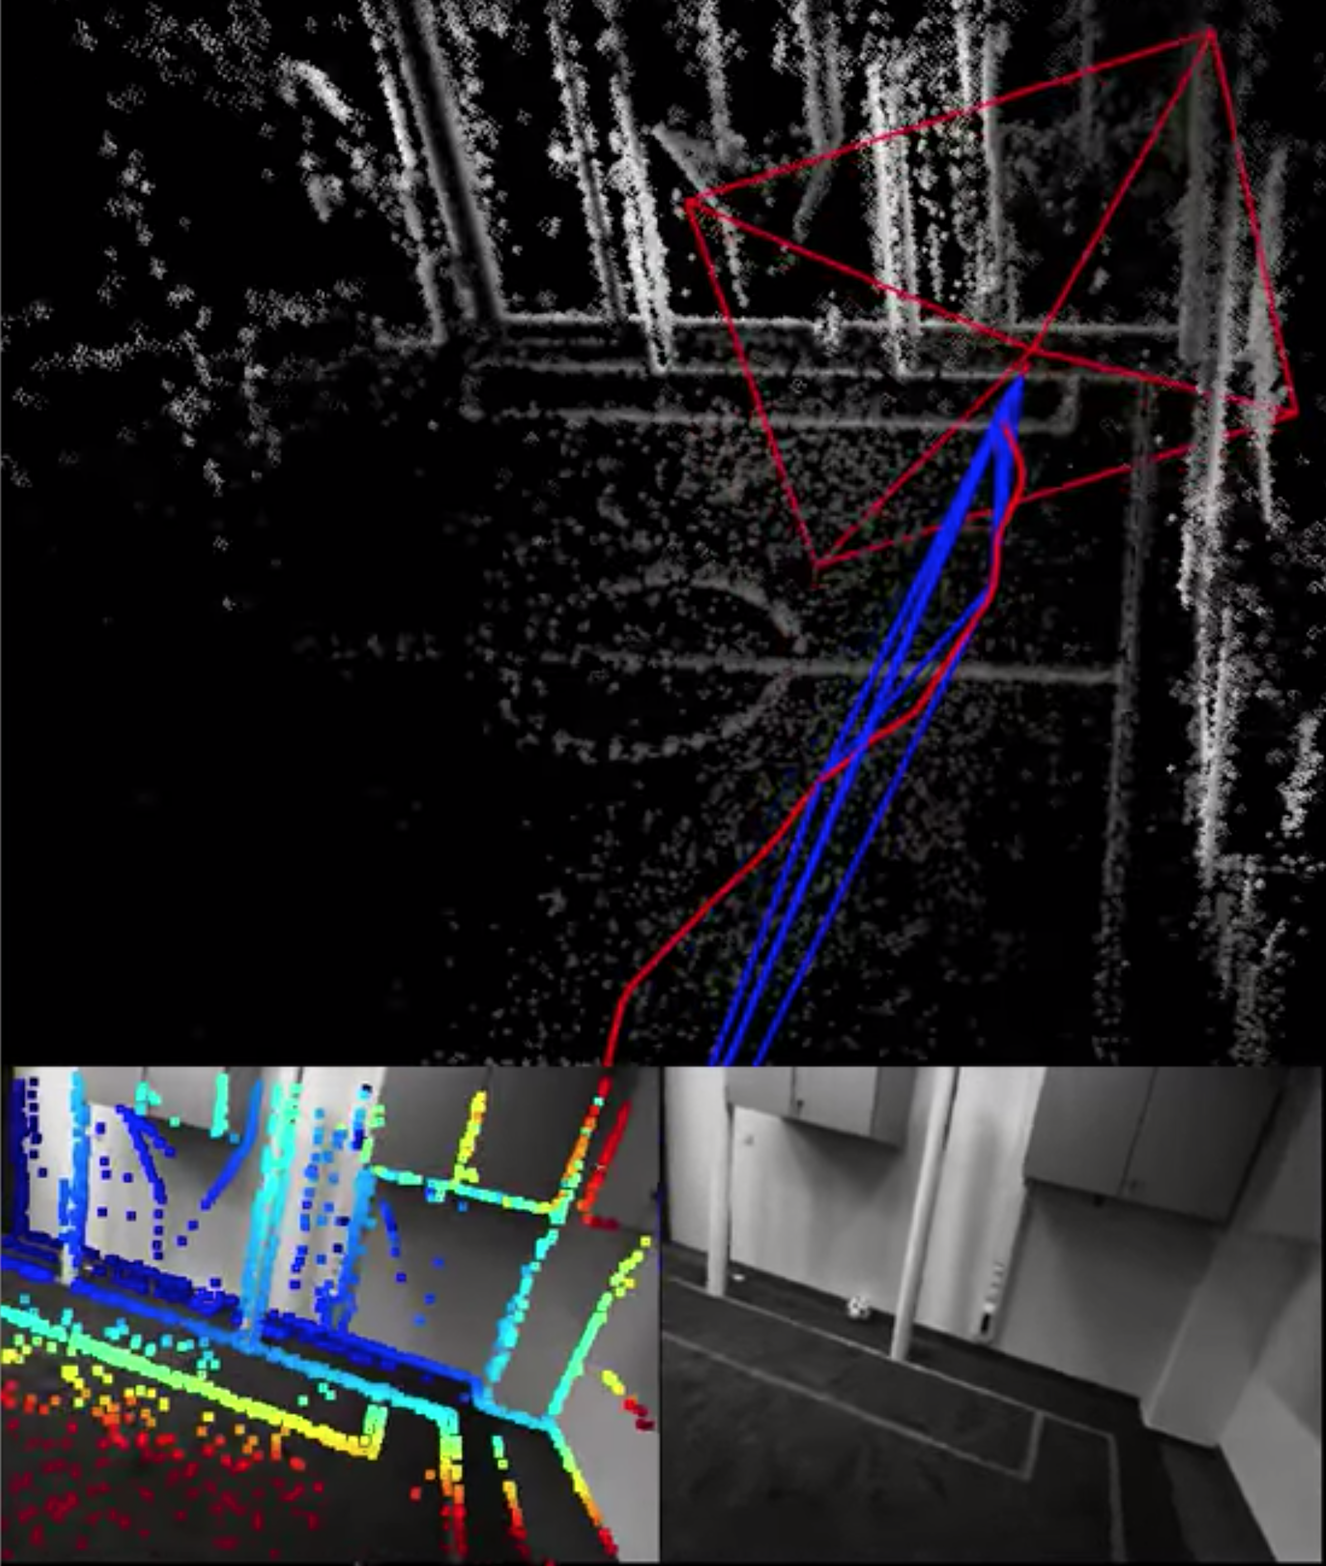
\includegraphics[width=0.5\linewidth]{dso}\vspace{-1ex}
	\caption{ Output sample of DSO on soccer field.}
	\label{FigDSO}
\end{figure}


\subsubsection{Dynamic Model Calibration}
Most of the information used for localization relies on information provided by the camera. 
Having the exact kinematic model of the robot is not always possible. 
Therefore it is necessary to calibrate variations from the designed CAD model to prevent potentially large projection errors for distant objects. 
A calibration of the kinematics on each robot that tunes translation and rotation offsets between the torso and the camera is required. 
These offsets are crucial for a good performance of the pixel to egocentric coordinate projection algorithm.
During the last years, multiple teams have started to work on automatic kinematic calibration. 
These approaches are generally based on the use of visual markers easily detectable such as Aruco Tags~\cite{Garrido-Jurado2014}.

%\subsubsection{Verbal Communication}
%OPT:talk about coach and referee understanding

%\subsection{Decision-making}
%OPT: write paragraph about decision-making under uncertainty

%\subsection{Interaction with humans}
%OPT: write about safety and natural aspect of soccer playing

\section{\label{sec:ShortTerm}Short-term: upcoming changes}

\subsection{RoboCup 2019 changes}

The major rule changes for RoboCup 2019 are as following:

\begin{itemize}
\item Natural lightning conditions are now explicitly allowed.
  It provides more flexibility for the local organizers and
  helps to prepare for moving outdoors while stimulating research on perception.
  Since SPL has already had some success in these conditions,
  it is reasonable to expect teams to be able to adapt.
\item Throw-in, corner kicks and goal kicks will be introduced.
  This will make games closer to FIFA games,
  thus making it easier for public to understand referee's interventions on the field.
  It is also expected that this will encourage teamplay since stoppage of games
  allow robots to position themselves.
\item The rules with respect to pick-up of robots and penalties for invalid
  behavior have been reworked to reduce the number of interventions from the referees.
  It also encourages team to have robust robots playing during the whole game by
  increasing constraints on penalized robots.
\item The presence of an emergency stop button will be required but without
  constraints on appearance.
  It is a mandatory step toward allowing robots to play with humans.
\item For the adult size league, the size of the field increases to
  $14 \times 9$ meters (previously $9 \times 6$ meters)
  and the games are now played 2 vs 2 robots.
  These changes will allow teamplay options for this league and is taking into
  account the fact that the locomotion speed for this league has significantly
  evolved for the past few years.
\end{itemize}

There are also some minor adjustements:

\begin{itemize}
\item Time for repositioning during some stoppage of game has been increased.
  In 2018, several teams had trouble to reach their own half within the time
  constraints after scoring a goal.
  This led to frequent interventions from handlers which can be reduced by
  slightly increasing the time allowed for robots to position autonomously
  during stoppage of games.
\item A new phrasing regarding constraints on foot design has been introduced to
  reduce the risk of misunderstandings.
\item The surface of teams markers is increased and the restriction regarding
  location of the markers on the robot have been reduced.
  This change will make it easier to detect opponents,
  thus improving the chances of presenting a satisfying gameplay to the public.
\end{itemize}

\subsection{RoboCup 2020 changes}

The process of updating the roadmap allowed to identify immediate changes which
could benefit the humanoid league.
One of the most important element is the organization of the league. Since 2010,
the league is composed of 3 leagues, KidSize, TeenSize and AdultSize.
While this structure was adapted at that time, evolution of the field and of the
teams at the RoboCup over the past years show that there are way for improvements.

For RoboCup2020, we intend to bring major modification to the league structure
in order to achieve the following objectives:
allow more diversity in the league,
increase the coherency of the structure with actual status of the competition
and finally propose a more flexible structure which can be easily adapted.

The scheduled changes are as follows:
\begin{itemize}
\item Restructuring regular tournament
\item Open Humanoid Leagues
\item Humanoids Demo Events
\item Reduction of the handlers interventions
\item Update of the technical challenges
\end{itemize}

This section starts by describing the changes and then summarize the impacts on
organization.

% TODO add emergency button (safe robotics) ?

\subsubsection{Restructuring regular tournament}

While the number of teams involved in the TeenSize league has globally increased
since 2010, the height of the robots in this league is globally decreasing and
entering the buffer zone between KidSize (max 90cm) and TeenSize(min 80cm).
\begin{description}
\item[RoboCup 2017:] 5 teams had robots larger than 90cm.
\item[RoboCup 2018:] Only 1 team had a robot above 90cm (94cm).
\item[RoboCup 2019:] According to the qualification material, all teams have
  robots between 80 and 90cm.
\end{description}

In regard of these elements, we propose to integrate the small robots from
TeenSize to the KidSize and the larger robots to the AdultSize.

Increasing the number of participants in each league would also make it easier
to separate the main league in two divisions, allowing experienced teams to have
more competitive games and new teams to have a more interesting event.
It would also be interesting to increase the average number of robots on
the pitch without loosing teams du to financial issues.
Finally, while Drop-In games has triggered the interest of multiple teams,
some teams find that it overloads the schedule, especially during the knock-out
phases.

In order to solve these problems, the tournament will use the following
structure:
\begin{enumerate}
\item The tournament will start by all the Drop-In games. This phase will
  require only one robot per team.
\item Teams who have not the maximum number of robots allowed for their league
  are required to form combined teams in order to form a full team of robots.
\item If there are less than 16 teams in the league after the merge procedure,
  all teams play in division A.
  If there are more than 16 merged teams, repartition of the teams is based
  on the result of the teams during Drop-In games and play-off games.
  \begin{description}
  \item[Division A:] Best 6 teams + winners of play-offs for teams 7-10.
  \item[Division B:] Losers from play-offs teams 7-10, teams 11-20,
    winners of play-offs for teams 21-28.
  \end{description}
\end{enumerate}

This structure ensures that teams who have a single robot can participate and
play a fair number of games.
Teams with more resources are allowed to present a full team in order to work
on their teamplay during the year.
Finally, this method ensures that the fields will have the appropriate number
of robots, from the Drop-In to the regular tournaments.

\subsubsection{Open Humanoid Leagues}

Current implementation as led to some constraints on robot design~(passive
sensors, size limitations) and complex rules in order to ensure fair games and
to focus on human-like structure and perception.
While this allows to bring the rules of the competition closer to the FIFA rules,
it increases the entry cost for newcomers.
In order to attract new teams, the Open Humanoid League will be opened.
This league will have a very limited number of rules and reduced hardware constraints.

Since it is difficult to anticipate how many teams will apply for this league,
implementation details will be chosen depending on the teams interested by this
competition.
Trophies will be awarded to the teams according to the same rules as regular leagues.

\subsubsection{Humanoids exhibition events}

Increasing the diversity of approaches used inside the league and broadening the
views of participants is important to avoid stagnation and uniformity in design.
In order to reduce this risk, exhibition events will be introduced.

Each year, research themes relevant to the league will be chosen by the TC.
Both, teams from the RoboCup and research teams in robotics will be
invited and selected to present their work during the RoboCup.

Demonstrations will not be limited to soccer playing humanoid robots, they will
also include innovation on specific themes (e.g. soft robotics).
The aim is to reserve space and time slots to present innovation in technology
or research in order to stimulate apparition of new ideas in the league.
Constraints on the exhibitions will be avoided in order to allow original
elements, no awards will be provided in order to keep it as a competition-free
event.

\subsubsection{Reducing handlers interventions}
% Presence of handlers -> less autonomy/robustness + less interesting for public
Presenting autonomous robots performing complex tasks is one of the strength of
the RoboCup community.
In this context, every opportunity to move robots on the field given to handlers
reduces the constraints on autonomy and therefore the achievement.
Moreover, interactions of the handlers with the robots reduces the interest from
the public.

Currently, handlers are allowed to place manually a striker and a goalie.
In 2020, all robots will have to perform autonomous placement,
starting from the side of the field.
The aim of this change is to focus on autonomy and robustness in localization
while reducing the frequency of human interventions.

\subsubsection{Update of the technical challenges}

From 2020, it will be mandatory for teams to have multiple robots in their team
or to merge with other teams for the regular tournament.
Therefore, we will start introducing technical challenges requiring collaboration between robots.

One of the current challenges is based on performing a kick on the goal from a moving ball.
Currently, the pass can be performed by either a robot or a human.
In 2020, pass will have to be performed by a robot.
By enforcing this as a technical challenge we intend to promote dynamic gameplay.

The high-jump challenge will be changed toward a landing challenge which will
focus on absorbing shocks and thus on soft robotics.

On the same trend, a standing-up challenge will be introduced for adult size robots.
This technical challenge will then evolve toward falling robots with the aim of removing
robot handlers on the long-term.


\section{\label{sec:LongTerm}Long-term: event triggered roadmap}

% TODO: Reminder of the reason pushing toward event-triggered roadmap

% TODO: Description of structure of the document

\subsection{Guiding principles}

% Events or measures are used to trigger the changes
Changes in the rules will be triggered by either research breakthrough or
continuous improvement of some skills. Those improvements will be ensured
through either measures of metrics during the game such as walking speed or
success at technical challenges. This will ensure that the rules improvements
are coherent with the capabilities of the robots in the league.

% Triggered changes apply with a delay, useful for teams and LOC
During the roadmap workshops and the polls, several teams requested to have
updates rules known sooner, in order to plan their development for the
competition. Similar issues arise for local organization with changes regarding
the size of the fields. In order to provide more time to teams and local
organizers while still allowing adaptation of the rules, we propose to separate
the evolution of the league in three categories depending on the number of years
required between announcement of the rule change and its application. Note that
we consider a 4 month period to allow the TC to implement the changes inside the
rulebook.
\begin{description}
\item[1Y:] Changes which can be done from one competition to the other without
  requiring previous announcement. This is limited to rule changes which have
  low impact on the robot design and do not require additional space for the
  competition. These changes have to be announced at least 8 months prior
  to the competition.
\item[2Y:] Changes which might require significant hardware investment for the
  teams or important modifications for the local organizers. These changes have
  to be announced at least 20 months prior implementation.
\item[4Y:] Major changes which require drastic modifications on robot design.
  These changes shave to be announced at least 44 months prior to the
  competition.
\end{description}

\subsection{\label{sec:metrics}Metrics used}
Continuously assessing the performances of the robots is a crucial point to
ensure that evolution of the rules is consistent with the improvements of the league.
Another benefit of gathering metrics on the performance of the robots is the possibility to
measure the impact of rule changes and the progress made.

In order to capture the performances of the robot during the games, we propose
to record logs of the game including: videos, messages from the referee box and
messages from the robots.
Teams will be strongly encouraged to share information on the perception and
intention of their robots which is a required element to assess their performance.
Ground truth will be obtained by human annotation of multiple calibrated video streams.

Gathering the metrics presented in this section will strongly improve the
possibilities to assess improvements in the league, allow teams to publish
quantitative results to support their claims and provide large amount of data
to run learning algorithms.
However, those benefits will come at a cost:
significant software development will be required,
human effort will be needed to validate the data and teams will have to agree on
a common protocol.
Therefore, extraction of the metrics will be introduced progressively during the
next years.


\subsubsection{Motion metrics}

\begin{description}
\item[Peak speed:] Reaching high-speed bipedal locomotion is one of the key
  research theme of the league.
  This measure is based on the highest distance traveled by a robot over 5 seconds.
  
\item[Approach time:] Efficiently controlling a locomotion engine based on perception
  is a difficult problem.
  The time required to travel the last meter before kicking is a good indicator
  of its controllability.

\item[Kicks and throw-ins:] Kicking the ball in soccer is one of the most important
  skills.
  From a robotic point of view, kicking is a highly dynamic motion task where
  a maximum of energy has to be transmitted to the ball while keeping balance
  and preserving accuracy.
  Keeping track of the different types of kicks and some of their properties helps
  to better understand the evolution of the game
  \begin{description}
  \item[Kick type:] There are many different types of kicking in soccer:
    forward kicks, side kicks, heel kicks, throw-ins (with hands) and even bicycle.
  \item[Ball status:] Robots can kick in ball which are static, rolling or
    flying at the moment of the impact.
    The number of kick from rolling balls or flying balls is a strong indicator
    of the dynamics of the games.
  \item[Kick power:] Powerful kicks give a strong incentive toward teamplay.
    This measure is based on the distance traveled by the ball before stopping or bouncing.
  \item[Kick accuracy:] In order to play as a team or to score goals, it is
    important that robots are capable of kicking accurately.
    Measuring the difference between intention of the robot and the result of his kick with
    respect to direction and power helps to assess the quality of kicks.
  \item[Execution-time:] Smooth transition between motions is an important research theme.
    Time required to go from walking motion to the end of the kick motion measures both,
    the transition and the dynamic aspect of the motion.
  \end{description}
\end{description}


\subsubsection{Perception metrics}

The comparison between ground truth and belief of the robot will allow to measure
the quality of the perception of the robots.

\begin{description}
\item[Ball Localization and prediction:] The measure of ball localization takes
  into account the percentage of time where the ball is located and the
  quality of the position estimation in an egocentric basis.
  On long-term, estimation of the speed of the ball and prediction of the trajectory will
  be considered.
\item[Self Localization:] Accurate localization in natural environment is a
  difficult problem which include detection of features, odometry and filtering.
  It is an essential skill for teamplay and high-level behaviors.
  The measure of self-localization includes position and orientation of the robot
  on the field.
\item[Opponent recognition:] Measure of the quality of opponent recognition will
  be based on estimated position and orientation of the opponents in an egocentric
  basis.
  On long-term, recognition of other robots intentions will also be evaluated.
\end{description}

\subsubsection{Gameplay metrics}

High-level metrics related to gameplay are used to measure global performances
of the teams and the quality of the teamplay.

\begin{description}
\item[Shots on goal:] The number of shots on goal during each game.
\item[Diving saves:] The number of successful and failed dives from goalies.
\item[Robots on field:] The average number of robots on the field per team
  during games can be compared with the maximum number of robots authorized
  in order to estimate robustness.
\item[Don't Mess Up Period (DMUP):] The DMUP is another robustness measure which indicates the
  level of autonomy of the robots.
  The DMUP is the period during which a robot played fully autonomously.
  Increasing the DMUP is a preliminary to remove the handlers.
\end{description}


\subsection{Detailed rule changes}
This section presents briefly recent and future evolutions of the rules of the
competition.
It can be used to have an overview of the path traveled recently and on the
steps remaining to reach the 2050 goal.
For past evolutions and short-term changes, the year of the introduction of the
change is indicated.
For long-term changes, the conditions required to implement the changes and the
delay between announcement of the change and its application are indicated.
Conditions for changes are based on the metrics presented in section~\ref{sec:metrics}.
In order to ensure competition is viable for multiple teams,
at least 3 teams need to fulfill the conditions to trigger the changes.

\subsubsection{Field evolution and number of robots}
% Importance of field and #robots for research and for accessibility for the teams
Playing on real soccer fields with eleven humanoid robots per team is a
long-term challenge which requires multiple breakthrough in research,
particularly in locomotion.
On the other hand, there are also technical and financial concerns:
few teams are able to train on an entire field due to the space constraints and
building eleven robots per team would be too expensive.

% Last evolutions
Since the beginning of the league, the number of robots per team has been increasing slowly
and several changes have been made to the fields:
\begin{itemize}
\item The size has increased with the walking speed of the robots.
\item While the initial fields contained extra information, those elements have
  been progressively removed, causing a shift in methods used for ball
  detection and localization.
\item Introduction of artificial turf has proven to be a major challenge for
  locomotion and has led to original hardware solutions to tackle the problem~\cite{Passault2015}.
  It has also strongly reduced the distance traveled by the ball when kicking,
  thus putting more constraints on shoots.
\end{itemize}

% Upcoming changes
Since bipedal locomotion is one of the main reasearch theme of the league,
increasing the size of the field in order to match the increasing speed of the
robots will be required.
In order to keep the gameplay interesting,
it is mandatory to ensure that the size of the field stays coherent with the
capacities of the robots.
Further increases in the size of the field will allow to have more robots on the pitch,
a crucial aspect to encourage collaboration between robots.

The roadmap for evolution of the field and the number of robots per team
is presented in Fig.~\ref{fig:field_dimensions}.
Changes will be triggered by the following conditions: robots should be able to cross
the current field in 20 seconds and they should be able to kick the ball across half the field.
Due to the major impact of field changes to the organization of the event,
changes with respect to the size of the field need to be announced 2 years prior to application.

% TODO: add outdoor?
\begin{figure}[htb]
  \centering
  \tikzstyle{element}=[rectangle, draw=black, rounded corners, text centered,
  anchor=north, text width=2cm, minimum height= 1cm]
\tikzstyle{fake}=[rectangle, text centered, anchor=north, text width=2cm, minimum height= 1cm]
\tikzstyle{league}=[rectangle, rounded corners, text width=4cm,
  anchor=north, minimum height= 1cm, font=\bfseries]
\tikzstyle{transitionNote}=[rectangle, right, rounded corners, %text left,
  text width=4cm, minimum height= 1cm]
\tikzstyle{horizontalTransitionNote}=[rectangle, above, rounded corners, midway, %text center,
  text width=0.5cm, minimum height= 1cm]
\tikzstyle{dependency} = [->, thick]

\begin{tikzpicture}[node distance=1cm, every node/.style={scale=0.6}]
  \node (Teen-2vs2-6by4) [element] {2 vs 2\\$6 \times 4$}; 
  \node (Teen-2vs2-9by6) [element,below=of Teen-2vs2-6by4] {2 vs 2\\$9 \times 6$}; 
  \node (Teen-3vs3-9by6) [element,below=of Teen-2vs2-9by6] {3 vs 3\\$9 \times 6$};
  \draw [dependency] (Teen-2vs2-6by4)  edge node [transitionNote] {2011} (Teen-2vs2-9by6);
  \draw [dependency] (Teen-2vs2-9by6)  edge node [transitionNote] {2017} (Teen-3vs3-9by6);
  
  \node (Kid-2vs2-45by3) [element,left=2cm of Teen-2vs2-6by4] {2 vs 2\\$4.5 \times 3$};
  \node (Kid-3vs3-6by4) [element,below=of Kid-2vs2-45by3] {3 vs 3\\$6 \times 4$}; 
  \node (Kid-4vs4-9by6) [element,below=of Kid-3vs3-6by4] {4 vs 4\\$9 \times 6$}; 
  \node (Kid-6vs6-14by9) [element,below=of Kid-4vs4-9by6] {6 vs 6\\$14 \times 9$}; 
  \node (Kid-8vs8-21by14) [element,below=of Kid-6vs6-14by9] {8 vs 8\\$21 \times 14$}; 
  \node (Kid-11vs11-32by21) [element,below=of Kid-8vs8-21by14] {11 vs 11\\$32 \times 21$};
  \draw [dependency] (Kid-2vs2-45by3)  edge node [transitionNote] {2008} (Kid-3vs3-6by4);
  \draw [dependency] (Kid-3vs3-6by4)  edge node [transitionNote] {2014} (Kid-4vs4-9by6);
  \draw [dependency] (Kid-4vs4-9by6) edge node [transitionNote] {2Y:\\peakSpeed $>$ 0.45 $m/s$\\kickDist $>$ 4.5 $m$} (Kid-6vs6-14by9);
  \draw [dependency] (Kid-6vs6-14by9) edge node [transitionNote] {2Y:\\peakSpeed $>$ 0.7 $m/s$\\kickDist $>$ 7 $m$}  (Kid-8vs8-21by14);
  \draw [dependency] (Kid-8vs8-21by14) edge node [transitionNote] {2Y:\\peakSpeed $>$ 1.05 $m/s$\\kickDist $>$ 10.5 $m$} (Kid-11vs11-32by21);

  \node (Adult-start) [fake,right=1cm of Teen-2vs2-6by4] {}; 
  \node (Adult-1vs1-9by6) [element,below=of Adult-start] {1 vs 1\\$9 \times 6$}; 
  \node (Adult-2vs2-14by9) [element,below=of Adult-1vs1-9by6] {2 vs 2\\$14 \times 9$}; 
  \node (Adult-3vs3-21by14) [element,below=of Adult-2vs2-14by9] {3 vs 3\\$21 \times 14$}; 
  \node (Adult-4vs4-32by21) [element,below=of Adult-3vs3-21by14] {4 vs 4\\$32 \times 21$};
  \node (Adult-6vs6-43by32) [element,below=of Adult-4vs4-32by21] {6 vs 6\\$43 \times 32$};
  \node (Adult-8vs8-65by43) [element,below=of Adult-6vs6-43by32] {8 vs 8\\$65 \times 43$};
  \node (Adult-11vs11-105by70) [element,below=of Adult-8vs8-65by43] {11 vs 11\\$105 \times 70$};
  \draw [dependency] (Adult-start) edge node[transitionNote] {2010} (Adult-1vs1-9by6);
  \draw [dependency] (Adult-1vs1-9by6) edge node[transitionNote] {2019} (Adult-2vs2-14by9);
  \draw [dependency] (Adult-2vs2-14by9)
        edge node [transitionNote] {2Y:\\peakSpeed $>$ 0.7 $m/s$\\kickDist $>$ 7 $m$}
        (Adult-3vs3-21by14);
  \draw [dependency] (Adult-3vs3-21by14)
        edge node [transitionNote] {2Y:\\peakSpeed $>$ 1.05 $m/s$\\kickDist $>$ 10.5 $m$}
        (Adult-4vs4-32by21);
  \draw [dependency] (Adult-4vs4-32by21)
        edge node [transitionNote] {2Y:\\peakSpeed $>$ 1.6 $m/s$\\kickDist $>$ 16 $m$}
        (Adult-6vs6-43by32);
  \draw [dependency] (Adult-6vs6-43by32)
        edge node [transitionNote] {2Y:\\peakSpeed $>$ 2.15 $m/s$\\kickDist $>$ 21.5 $m$}
        (Adult-8vs8-65by43);
  \draw [dependency] (Adult-8vs8-65by43)
        edge node [transitionNote] {2Y:\\peakSpeed $>$ 3.25 $m/s$\\kickDist $>$ 32.5 $m$}
        (Adult-11vs11-105by70);

  % Environment information
  \node (Enriched) [element,right=2cm of Adult-start] {Side Poles};
  \node (ColorCoded) [element,below=of Enriched] {Colored objects};
  \node (HumanLike) [element,below=of ColorCoded] {No colors};
  \draw [dependency] (Enriched) edge node [transitionNote] {2010: Restart marks\\2012: Side poles\\2013: Yellow goals} (ColorCoded) ;
  \draw [dependency] (ColorCoded) edge node [transitionNote] {2015:\\White goals\\White ball} (HumanLike);

  % Ground type
  \node (Carpet) [element,right=2cm of Enriched] {Carpet};
  \node (Turf) [element,below=of Carpet] {Artificial turf};
  \node (SoccerGrass) [element,below=of Turf] {Soccer field surface};
  \draw [dependency] (Carpet) edge node [transitionNote] {2015: 30mm turf} (Turf);
  \draw [dependency] (Turf) -- (SoccerGrass);


  % Cross league dependency
  \draw [dependency] (Teen-3vs3-9by6)  edge node [horizontalTransitionNote] {2020} (Kid-4vs4-9by6);
  \draw [dependency] (Teen-3vs3-9by6)  edge node [horizontalTransitionNote] {2020} (Adult-2vs2-14by9);

  % Categories
  \node (Kid) [league,text=black] at ($(Kid-2vs2-45by3) + (0.5,1.0)$) {Kid};
  \draw [draw=black] ($(Kid-11vs11-32by21) - (0.8,0.5)$) rectangle ($(Kid) + (1.9,0.2)$);
  \node (Teen) [league,text=black] at ($(Teen-2vs2-6by4) + (0.5,1.0)$) {Teen};
  \draw [draw=black] ($(Teen-3vs3-9by6) - (0.8,0.5)$) rectangle ($(Teen) + (0.3,0.2)$);
  \node (Adult) [league,text=black] at ($(Adult-start) + (0.5,1.0)$) {Adult};
  \draw [draw=black] ($(Adult-11vs11-105by70) - (0.8,0.5)$) rectangle ($(Adult) + (1.9,0.2)$);
  \node (FieldInformation) [league,text=black] at ($(Enriched) + (0.5,1.0)$) {Field Information};
  \draw [draw=black] ($(HumanLike) - (0.8,0.5)$) rectangle ($(FieldInformation) + (1.9,0.2)$);
  \node (FieldSurface) [league,text=black] at ($(Carpet) + (0.5,1.0)$) {Field Surface};
  \draw [draw=black] ($(SoccerGrass) - (0.8,0.5)$) rectangle ($(FieldSurface) + (1.9,0.2)$);
  
\end{tikzpicture}

%TODO: add removal of magnetometer ?

  \caption{\label{fig:field_dimensions}Evolution of field and number of robots, dimensions in meters.}
\end{figure}

\subsubsection{Handlers and game duration}
% Robustness + Energy efficiency
Activity of the handlers and duration of half-times are related to three important research themes:
autonomy of the robots, robustness and energy efficient locomotion.
This section presents the roadmap along with some motivations,
Fig.~\ref{fig:handlers+game_duration} summarizes those evolutions.

% StandUp autonomous for adult
In KidSize and TeenSize, robots are requested to be able to fall and stand-up autonomously,
a prerequisite to remove constant presence of handlers on the field which is a
key point regarding autonomy for humanoid robots.
For AdultSize robots, falling and standing-up is an important research question,
while it is necessary to push toward this direction, it is not mature yet.
Incentive towards improvements on this topic will be given through technical challenges.
Once the problem has been tackled, requirements will be added to the rules and
handlers will not be allowed nearby robots.

% Robustness / long-term autonomy
For robots able to fall and stand-up autonomously,
the main challenge for autonomy is to reduce the frequency of human interventions in the league.
This implies constraints on the robustness of both, software and hardware.
Currently, several teams are relying on the possibility to pick-up robots every few minutes
to reset their status.
In order to create a higher incentive for robustness, it is necessary to have harsher penalties
for Pick-Up.
However, stricter rules would risk to result with less robots on the field which would not be
suitable for the public.
Therefore, before changing the rules, a minimum value of DMUP should be ensured.

% Game period
Once interventions of handlers are reduced to a minimum and robots are capable to play autonomously,
increasing the duration of half-time will bring high incentive toward energy efficient locomotion.
In order to ensure that increases of the duration are coherent with capacities of the robots,
it will be required that teams can play at least the half a period without intervention
from the handler in average before increasing time duration.

\begin{figure}
  \centering
  \tikzstyle{element}=[rectangle, draw=black, rounded corners, text centered,
  anchor=north, text width=4cm, minimum height= 1cm]
\tikzstyle{fake}=[rectangle, text centered, anchor=north, text width=2cm, minimum height= 1cm]
\tikzstyle{league}=[rectangle, rounded corners,
  anchor=north, minimum height= 1cm, font=\bfseries]
\tikzstyle{transitionNote}=[rectangle, right, rounded corners, %text left,
  text width=6cm, minimum height= 1cm]
\tikzstyle{horizontalTransitionNote}=[rectangle, above, rounded corners, midway, %text center,
  text width=0.5cm, minimum height= 1cm]
\tikzstyle{dependency} = [->, thick]

\begin{tikzpicture}[node distance=1cm, every node/.style={scale=0.6}]
  \node (HandlersOnPitch) [element] {Handlers on pitch}; 
  \node (TC-StandingUp) [element, below=of HandlersOnPitch] {Technical Challenge:\\Standing-Up}; 
  \node (TC-Falling) [element, below=of TC-StandingUp] {Technical Challenge:\\Falling};
  \node (HandlersOut) [element, below=of TC-Falling] {Handlers out of field};
  \node (KidTeenStart) [fake, below=of HandlersOut] {};
  \draw [dependency] (HandlersOnPitch)  edge node [transitionNote] {2020: Adult Size} (TC-StandingUp);
  \draw [dependency] (TC-StandingUp)  edge node [transitionNote] {StandUp $< 10s$} (TC-Falling);
  \draw [dependency] (TC-Falling)  edge node [transitionNote] {Fall on hard ground} (HandlersOut);
  \draw [dependency] (KidTeenStart)  edge node [transitionNote] {KidSize + TeenSize} (HandlersOut);
  
  \node (ManualPlacement) [element, right=1cm of HandlersOnPitch] {Autonomous placement:\\Optional};
  \node (HalfWayPlacement) [element, below=of ManualPlacement]
        {Autonomous placement:\\All but Goal+Striker};
  \node (AutonomousPlacement) [element, below=of HalfWayPlacement] {Autonomous placement:\\Required};
  \node (PickUpPenalty) [element, below=of AutonomousPlacement] {Pick-Up:\\Major penalty};
  \node (15minutes) [element, below=of PickUpPenalty] {Half-Time increase:\\15 minutes};
  \node (20minutes) [element, below=of 15minutes] {Half-Time increase:\\20 minutes};
  \node (30minutes) [element, below=of 20minutes] {Half-Time increase:\\30 minutes};
  \node (45minutes) [element, below=of 30minutes] {Half-Time increase:\\45 minutes};
  \draw [dependency] (ManualPlacement)  edge node [transitionNote] {2017} (HalfWayPlacement);
  \draw [dependency] (HalfWayPlacement)  edge node [transitionNote] {2020} (AutonomousPlacement);
  \draw [dependency] (AutonomousPlacement)  edge node [transitionNote] {2Y: avg(DMUP) > 3 minutes} (PickUpPenalty);
  \draw [dependency] (PickUpPenalty)  edge node [transitionNote] {2Y: avg(DMUP) > 5 minutes} (15minutes);
  \draw [dependency] (15minutes)  edge node [transitionNote] {2Y: avg(DMUP) > 7.5 minutes} (20minutes);
  \draw [dependency] (20minutes)  edge node [transitionNote] {2Y: avg(DMUP) > 10 minutes} (30minutes);
  \draw [dependency] (30minutes)  edge node [transitionNote] {2Y: avg(DMUP) > 15 minutes} (45minutes);

  \draw [dependency] (HandlersOut) -- (PickUpPenalty);
\end{tikzpicture}

%TODO: add removal of magnetometer ?

  \caption{\label{fig:handlers+game_duration}Evolutions regarding handlers and game duration}
\end{figure}

\subsubsection{Gameplay rules}
% Context
In order to reach the 2050 goal, robots have to be able to play according to
rules similar to the FIFA rules\footnote{It is inevitable to bring modifications
  to the rules, at least to impose some constraints on the size of the robots,
  see~\cite{Stone2010} for more details on relationship between rules of soccer
  and robotic soccer.}.
However, robots have to reach very high-level of autonomy in order to play according to soccer rules.
As example, respecting the offside rules is particularly challenging with respect to perception.

% Recent evolution
At the origin of the league,
the competition was centered around technical challenges and penalty shootouts.
Since 2006, the competition has moved toward real soccer games with rules tending
to get closer to the FIFA rules.
The latest implemented change is the introduction of goal kick, corner kicks and
throw-in or kick-in for RoboCup2019.

% Upcoming changes
There are 2 major gameplay changes remaining to have the gameplay rules similar to FIFA.
The first is enforcing that throw-in are performed using hands,
this rule will be introduced once the throw-in capacities are performed quickly and
strongly enough.
The second and most challenging remaining rule is the offside rule.
It will require to ensure that three keypoints are achieved:
Self-localization, localization of opponents and a minimum number of robots on the field.
Evolution and perspectives for the gameplay rules are shown in Fig.~\ref{fig:gameplay_rules}.

\begin{figure}
  \centering
  \tikzstyle{element}=[rectangle, draw=black, rounded corners, text centered,
  anchor=north, text width=4cm, minimum height= 1cm]
\tikzstyle{fake}=[rectangle, text centered, anchor=north, text width=2cm, minimum height= 1cm]
\tikzstyle{league}=[rectangle, rounded corners,
  anchor=north, minimum height= 1cm, font=\bfseries]
\tikzstyle{transitionNote}=[rectangle, right, rounded corners, %text left,
  text width=6cm, minimum height= 1cm]
\tikzstyle{horizontalTransitionNote}=[rectangle, above, rounded corners, midway, %text center,
  text width=0.5cm, minimum height= 1cm]
\tikzstyle{dependency} = [->, thick]

\begin{tikzpicture}[node distance=1cm, every node/.style={scale=0.6}]
  \node (Penalty) [element] {Penalty Shootouts};
  \node (Dribble) [element, below=of Penalty] {Dribble and Kick};
  \node (AdultStart) [fake, right=2cm of Dribble] {};
  \node (RegularGames) [element, below=of Dribble] {Regular games\\Simplified};
  \node (FreeKicks) [element, below=of RegularGames] {Regular games\\Free Kicks}; 
  \node (CornerKicks) [element, below=of FreeKicks]
        {Regular games\\Goal and Corner Kicks\\Throw-in or Kick-in}; 
  \node (ThrowIn) [element, below=of CornerKicks]
        {Regular games\\Throw-in mandatory};
  \node (Offside) [element, below=of ThrowIn]
        {Regular games\\Offside rule};

  \draw [dependency] (Penalty)  edge node [transitionNote] {2006: Teen Size} (Dribble);
  \draw [dependency] (Dribble)  edge node [transitionNote]
        {2006: Kid Size\\2010: Teen Size\\2017: Adult Size} (RegularGames);


  \draw [dependency] (AdultStart)  edge node [horizontalTransitionNote] {2010: Adult Size} (Dribble);
\end{tikzpicture}


  \caption{\label{fig:gameplay_rules}Evolutions of gameplay rules}
\end{figure}

%OPT: subsubsection for technical challenges?

\section{Evolution of the document}

Since breakthroughs in research and evolution of the games is very difficult to predict,
the following document should be frequently updated in order to match.
It should also be possible for the league and for the trustees to request for
modifications because some elements seems unrealistic with respect to the current
status of the league.

In order to highlight that the document need to be update frequently, we present
here the minimal frequency for updating the different sections of this document:
\begin{itemize}
\item Section~\ref{sec:ScientificChallenges} emphasizes on research related to
  the RoboCup Humanoid League and on contributions from the league.
  While major publications from the teams should be added to the document regularly,
  updating this section requires significant work from the TC and is based on
  global progress in research areas linked with the league.
  Next mandatory update is planned for 2024.
\item Section~\ref{sec:ShortTerm} presents upcoming changes in the rules.
  Since it has been made pretty clear by the team that updating the rulebook
  every year was too frequent,
  it is not mandatory to update it every year.
  Next mandatory update is planned for 2021.
\item Section~\ref{sec:LongTerm} presents the global evolution of the league.
  Since it includes metrics on the performance of the robots,
  it should be updated yearly, after each major competition.
  Next mandatory update is planned for 2020.
\end{itemize}

\newpage

\printbibliography


\end{document}
